
\section{Timeline for Data Facilities Implementation}\label{sec:timeline}
%Originally https://docs.google.com/document/d/1b9lk_bqxb2s6VOa94GQalRRXs1AYkFRYVDx1263RiHM/edit#

The timeline is derived from functionality required by the Data
Previews and then the first Data \gls{Release}, DR1. Analysis indicates that
the bulk of the service implementation is needed for \gls{DP1}, with the
exception of live alerts.

We need to develop a timeline for what needs done by when in the DFs, assuming something like mid 2023 to show everything is ready, if not scaled up already.
This would mean that everything in the scope document and derived services list would be deployed.

With \gls{DP0}.1 in progress, involvement with the Data Facilities will
begin with \gls{DP0}.2 \citedsp{RTN-001} following through to \gls{DP2}.
See also \gls{RDO}-011 for detail on the various Data Previews. Figure
\ref{timeline} shows the activities and events involved with
preparation for ComCam and DP1.

\begin{figure}
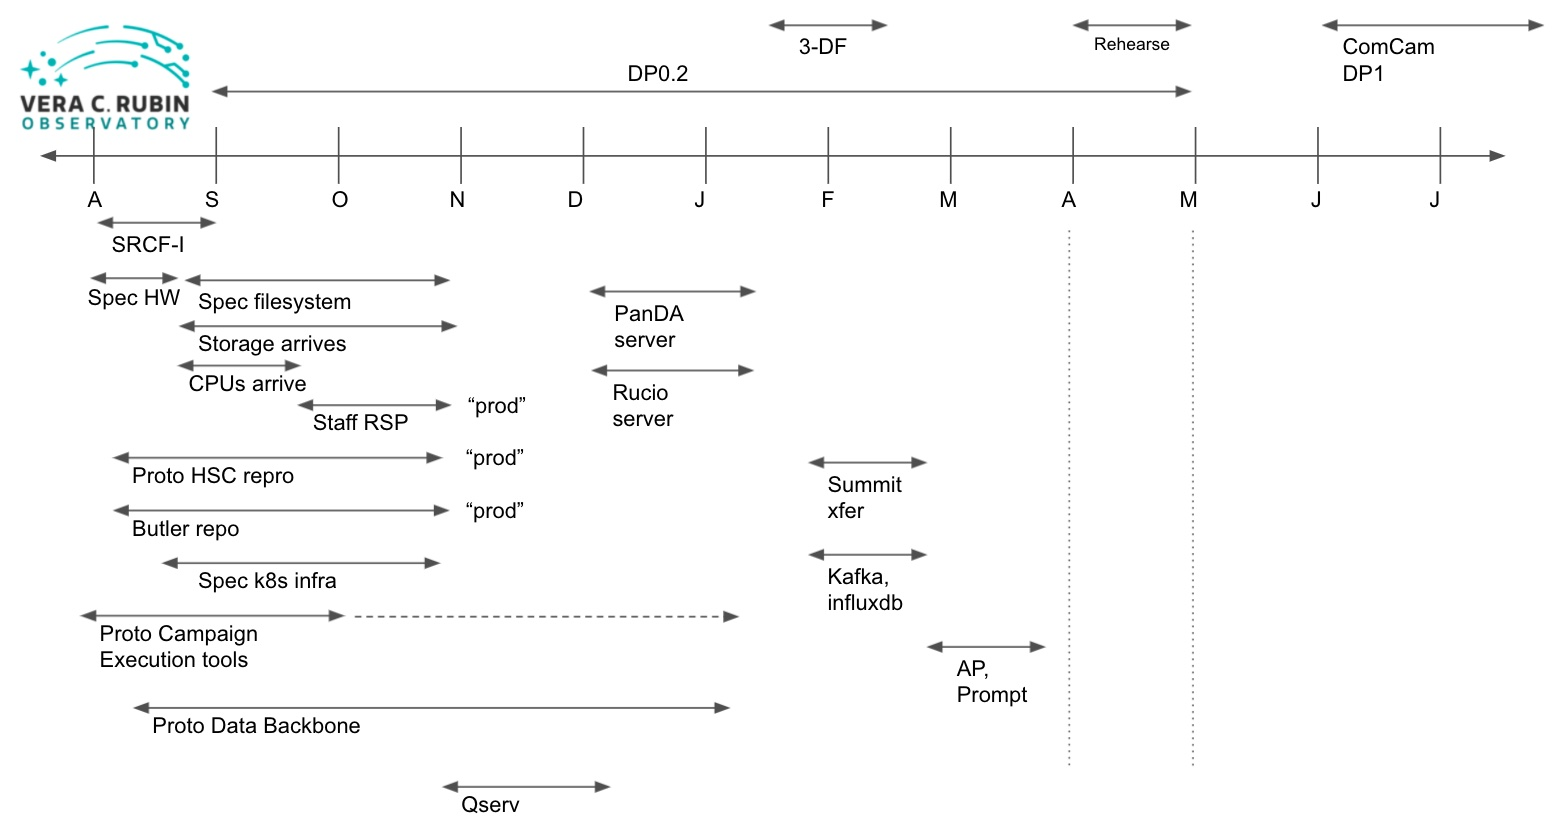
\includegraphics[width=\textwidth]{USDF-DP1_Timeline.jpg}
\caption{Timeline of DF Activities Supporting DP1 starting from August
2021}
\label{timeline}
\end{figure}

\begin{figure}
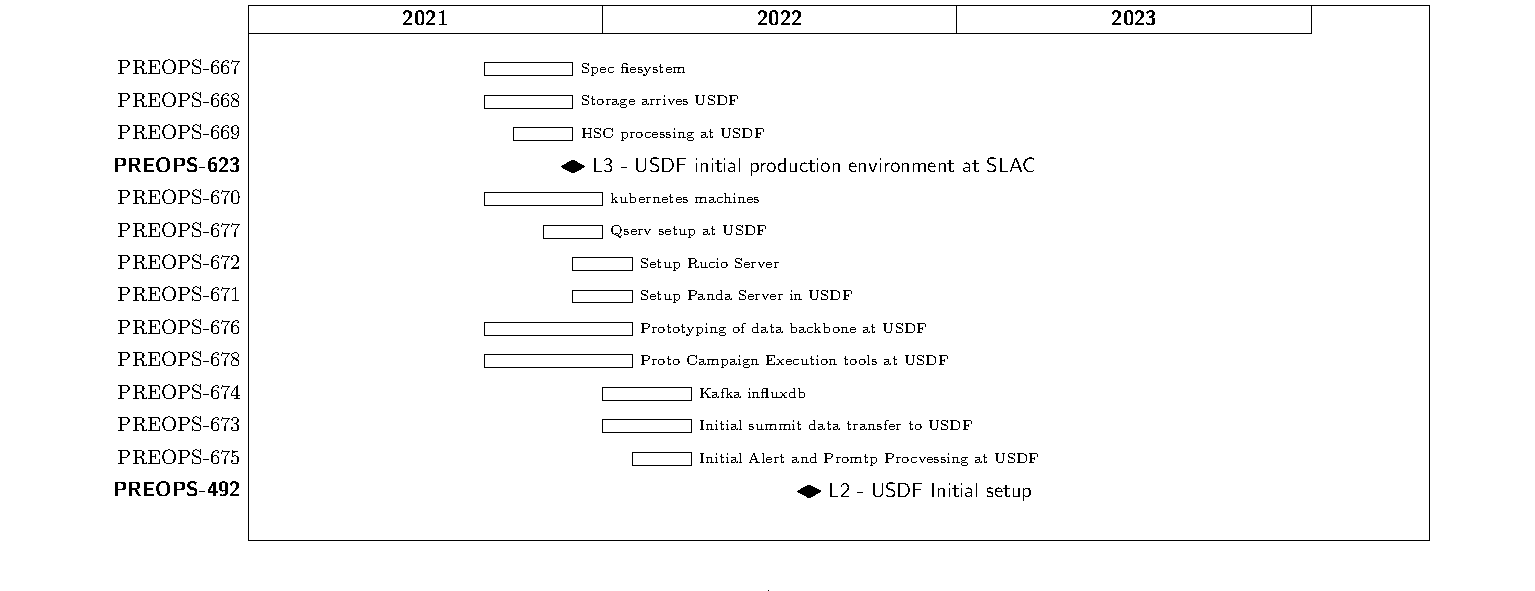
\includegraphics[width=0.7\textwidth]{USDFplan}]
\caption{Timeline of DF Activities Supporting DP1 - from Jira }
\label{gtimeline}
\end{figure}

The Data Production Milestones are listed in \tabref{tab:openMilestones} - we may need to add some more specifically for \gls{USDF}.
% This file was generated by opsMiles.py do not edit.
\tiny \begin{longtable} {|p{0.3\textwidth}  |r  |r  |r  |r |l |p{0.1\textwidth} |} \caption{Milestones for Rubin Observatory Data Production and System Performance  \label{tab:openMilestones}}\\ 
\hline 
{\bf Milestone}&{\bf Jira ID}&{\bf Rubin ID}&{\bf Due Date}&{\bf Level}&{\bf Status}&{\bf Team}\\ \hline 
PanDA based workflow system in place&\jira{PREOPS-154}&L3-MW-0050&2021-03-31&3&To Do&Science Users Middleware
 \\ \hline
Gen3 butler and pipeline task ready for DP0 production&\jira{PREOPS-156}&L3-MW-0070&2021-06-10&3&In Progress&Science Users Middleware
 \\ \hline
Engage with the community to support shared-risk simulated data distribution to community for science with DP0&\jira{PREOPS-150}&L2-SP-0020&2021-06-30&2&In Progress&Community Engagement
 \\ \hline
Science Platform ready on for DP0.2&\jira{PREOPS-157}&L3-PR-0040&2021-06-30&3&To Do&Science Platform and Reliability Engineering
 \\ \hline
PanDA based workflow system with tooling (e.g. restart) added.&\jira{PREOPS-155}&L3-MW-0060&2021-06-30&3&In Progress&Science Users Middleware
 \\ \hline
Evaluate Batch Production System &\jira{PREOPS-153}&L3-MW-0040&2021-07-31&3&To Do&Science Users Middleware
 \\ \hline
Demonstrate EPO interface with DP0&\jira{PREOPS-152}&L3-PR-0030&2021-09-30&3&To Do&Science Platform and Reliability Engineering
 \\ \hline
DP0.2 Early Access: Provide access to reprocessed images and visit level catalogs from the IDF&\jira{PREOPS-159}&L2-DP-0040&2021-09-30&2&To Do&Science Platform and Reliability Engineering
 \\ \hline
DP0.2 Reprocessing Start: Begin early DRP-like re-processing of DP0 simulated image data, at the IDF.&\jira{PREOPS-158}&L2-DP-0030&2021-09-30&3&To Do&Execution
 \\ \hline
Plan for how to use IN2P3 in DP0.2&\jira{PREOPS-160}&L3-EX-0010&2021-09-30&3&To Do&Execution
 \\ \hline
Deploy early instantiation of service desk providing second-tier technical support for community&\jira{PREOPS-147}&L3-PR-0020&2021-09-30&3&To Do&Science Platform and Reliability Engineering
 \\ \hline
Deliver initial Quality Assessment and Assurance (QA) plan for ComCam Data.&\jira{PREOPS-293}&FY20-0010&2021-10-30&2&To Do&Verification and Validation
 \\ \hline
Deliver preliminary implementation plan for real-time and daily monitoring&\jira{PREOPS-515}&L3-SC-0020&2021-12-31&3&To Do&Survey Scheduling
 \\ \hline
Deliver preliminary list of metrics for real-time and daily monitoring&\jira{PREOPS-514}&L3-SC-0010&2021-12-31&3&To Do&Survey Scheduling
 \\ \hline
 Deliver preliminary list of metrics for quarterly monitoring&\jira{PREOPS-517}&L3-SC-0040&2021-12-31&3&To Do&Survey Scheduling
 \\ \hline
Deliver LSST Data Products Documentation (DP0)&\jira{PREOPS-149}&L3-CE-0010&2022-03-31&3&In Progress&Community Engagement
 \\ \hline
L2 - DP0.2 Public release to delegates&\jira{PREOPS-483}&L2-DP-0051&2022-06-01&2&To Do&Data Production Management
 \\ \hline
L2 - DP0.2 Data Release: science-ready catalogs from reprocessed DP0 images released from the IDF&\jira{PREOPS-484}&L2-PF-0052&2022-06-30&2&To Do&System Performance Management
 \\ \hline
L2 - USDF Initial setup&\jira{PREOPS-492}&L2-DP-0081&2022-07-31&2&To Do&Infrastructure and Support
 \\ \hline
Deliver implementation of real-time and daily monitoring system&\jira{PREOPS-516}&L3-SC-0030 &2022-08-31&3&To Do&Survey Scheduling
 \\ \hline
 Deliver implementation of quarterly metric monitoring&\jira{PREOPS-518}&L3-SC-0050&2022-12-30&None&To Do&Survey Scheduling
 \\ \hline
L2 - Announce Initial Survey Strategy&\jira{PREOPS-490}&L2-SP-0060&2022-12-30&2&To Do&System Performance Management
 \\ \hline
\end{longtable} \normalsize


\subsection{Assumptions}

Nothing new is needed between \gls{DP2} and \gls{DR1}, except more
hardware. Each Data Preview is built on the previous one's functionality.

\subsection{Data \gls{Release} Productions}
\subsubsection{ \gls{DP0}.2 - \gls{DESC} DC2 reprocessing}
See \citeds{RTN-001}.
\begin{itemize}
\item start date: Q4 \gls{FY21}
\item end date: Q4 \gls{FY22}
\item Target: reprocess \gls{DC2} data on \gls{IDF}; run as first Ops rehearsal
\item Functionality:
\begin{itemize}
\item \gls{DRP}; \gls{DIA}; \gls{RSP}
\item \gls{PanDA} and Processing team driving processing
\item some campaign management
\item \gls{FrDF} planning parallel reprocessing and RSP; Probably not using
  \gls{PanDA}. May attempt some at \gls{USDF}:
\item run as Ops Rehearsal
\end{itemize}
\end{itemize}
\subsubsection{ Three Data Facility Rehearsal}
 As a precursor to DP1, a rehearsal involving all three Data
 Facilities is envisaged to demonstrate the ability to do multi-site
 processing:
 \begin{itemize}
\item local butlers which would contain the inputs and products of the processing done at each facility,
\item Rucio clients for triggering data replication among the facilities,
\item mechanism to accept jobs submitted by the PanDA
central instance for local execution
\end{itemize}
\subsubsection{ \gls{DP1} - ComCam}
\begin{itemize}
\item start date: Q3 \gls{FY22}
\item end date: Q2 \gls{FY23}
\item Target: at \gls{NCSA}; parallel processing at USDF; reprocessing at USDF, FrDF, UKDF
\item Released Products:
\begin{itemize}
\item full \gls{DRP}
\item \gls{AP}, but no live alerts.Canned alerts are planned to allow
  interactions with brokers and the \gls{MPC}.
\end{itemize}
\item Functionality:
\begin{itemize}
\item \gls{Summit} to \gls{USDF}  - dual path with NCSA
\begin{itemize}
\item transfer images
\item transfer calibrations - bidirectional
\item transfer \gls{EFD} contents
\end{itemize}
\item \gls{DF} production
\begin{itemize}
\item set up as processing site with sufficient storage and \gls{CPU};
  configurable clusters for AP vs DRP. PanDA server at \gls{SLAC}.
\item \gls{Qserv} + ingest mechanism
\item \gls{Butler} + ingest
\item \gls{RSP}
\item connection to brokers for canned alerts. (\gls{MPC}?)
\item Data movement among DFs
\item campaign management, \gls{monitoring} and quality assessment
\item IDACs may be under test at this phase
\end{itemize}
\end{itemize}
\item Resources needed
\begin{itemize}
\item Databases installed
\item \gls{EFD}, butler, \gls{PPDB}, APDB...
\item \gls{PanDA} server
\item \gls{Rucio} instance (?)
\item \gls{Qserv} size
\item \gls{CPU} \& storage
\end{itemize}
\end{itemize}
\subsubsection{DP2 - LSSTCam}
\begin{itemize}
\item start date: Q1 \gls{FY23}
\item end date: Q1 \gls{FY24}
\item Target: processing at \gls{USDF}; FrDF, UKDF
\item Released Products:
\begin{itemize}
\item full \gls{DRP}
\item \gls{AP}, with canned and live alerts.
\end{itemize}
\item Functionality in addition to \gls{DP1}:
\begin{itemize}
\item IDACs
\item Bulk downloads - including policy
\item Resources needed
\item \gls{CPU} + storage increases
\end{itemize}
\end{itemize}
\subsubsection{DR1 - Survey}
This is already operations.

\begin{itemize}
\item start date: Q3 \gls{FY24}
\item end date: Q1 \gls{FY25}
\item Released products
\begin{itemize}
\item full \gls{DRP}
\item \gls{AP} where templates are available, with some live alerts.
\end{itemize}
\item Functionality
\begin{itemize}
\item no additional functionality to \gls{DP2}
\end{itemize}
\end{itemize}
